% Machine translated from the Danish original, ../danish/ad-problems-2024-april.tex
% From the front page: CLRS refers to the 4th edition; some problems refer to online chapters from the 3rd edition that are not included in the 4th edition.
\noindent\emph{This problem set has been machine translated from the Danish original.}
\medskip

\section*{Multiple-choice}\label{sec:mc}

\placeholder{Where to enter the multiple-choice answers, e.g.\ the multiple-choice module of the exam system.}

\multiplechoicestart


\question{Sorting}
Consider a variant of {\sc Merge-Sort} that splits the input into \emph{three} parts of equal size (up to rounding), sorts each part recursively, and then merges the three parts with two calls to {\sc Merge} (CLRS Section 2.3). The pseudocode is as follows:
\begin{codebox}
  \Procname{$\proc{Merge3-Sort}(A, p, s)$}
  \li \If $p<s$ \Do
  \li $q = \lfloor (2\cdot p+ s)/3\rfloor$
  \li $r = \lfloor (p+2\cdot s)/3\rfloor$
  \li $\proc{Merge3-Sort}(A, p, q)$
  \li $\proc{Merge3-Sort}(A, q+1, r)$
  \li $\proc{Merge3-Sort}(A, r+1, s)$
  \li $\proc{Merge}(A, p, q, r)$
  \li $\proc{Merge}(A, p, r, s)$ \End
\end{codebox}

\noindent
Which recurrence describes the running time $T(n)$ of $\proc{Merge3-Sort}$ on an input of size~$n$ (where $n = s - p + 1$)?
\oneanswer
\optionsstart
\answer $T(n) = T(n/2) + \Theta(n)$
\answer $T(n) = T(2n/3) + \Theta(n)$
\answer $T(n) = 2\cdot T(n/3) + \Theta(n)$
\answer $T(n) = 2\cdot T(2n/3) + \Theta(n)$
\answer $T(n) = 3\cdot T(n/2) + \Theta(n)$
\answer $T(n) = 3\cdot T(n/3) + \Theta(n)$ \correct
\optionsend

\explanation{The three recursive calls each take time $T(n/3)$, while the two calls to {\sc Merge} take total time $\Theta(n)$.}




\question{Recurrences}
Which of the recurrences below, numbered $i=1,\dots,6$, have a solution $T_i$ with $T_i(n) = O(n^2)$?
Assume that $T_i(n) = 1$ for $n\leq 1$. \multipleanswers

\medskip\noindent
{\bf Examples.} If $T_0(n) = \Theta(n)$, then $T_0(n) = O(n^2)$ also holds. If $T_0(n) = \Theta(2^n)$, then $T_0(n) = O(n^2)$ does \emph{not} hold.

\optionsstart
\answer $T_1(n) = T_1(n/2) + \Theta(n^2)$ \correct
\answer $T_2(n) = 4\cdot T_2(n/2) + \Theta(n^2)$
\answer $T_3(n) = 3\cdot T_3(n/2) + \Theta(n)$  \correct
\answer $T_4(n) = T_4(n/3) + \Theta(n)$ \correct
\answer $T_5(n) = 2\cdot T_5(n/3) + \Theta(n)$ \correct
\answer $T_6(n) = 2\cdot T_6(n-2) + \Theta(n)$
\optionsend

\explanation{Recurrences 1--5 can be solved with the master theorem and have the solutions $T_1(n)=\Theta(n^2)$, $T_2(n)=\Theta(n^2\lg n)$, $T_3(n)=\Theta(n^{\lg_2 3})$, $T_4(n)=\Theta(n)$, and $T_5(n)=\Theta(n)$, respectively. Recurrence 6 can be solved as $T_6(n)=\Theta(2^{n/2})$ using the substitution method.}




\question{Lower bounds for sorting}
{\sc Merge-Sort} and (deterministic) {\sc Quicksort} as described in CLRS Sections 2.3 and 7.1 are examples of comparison sort algorithms.
Which conclusions can be drawn as a consequence of the lower bound for sorting, Theorem 8.1 in CLRS?
(You should not consider whether the conclusion is true, only whether it is a logical consequence of Theorem~8.1.)
\multipleanswers
\optionsstart
\answer There is an input on which {\sc Quicksort} runs in time $O(n \lg n)$ in the worst case
\answer There is an input on which {\sc Merge-Sort} runs in time $O(n \lg n)$ in the worst case
\answer There is an input on which {\sc Quicksort} runs in time $\Omega(n \lg n)$ in the worst case \correct
\answer There is an input on which {\sc Merge-Sort} runs in time $\Omega(n \lg n)$ in the worst case \correct
\answer On average over all inputs, {\sc Merge-Sort} runs in time $\Omega(n \lg n)$
\answer On average over all inputs, {\sc Quicksort} runs in time $O(n \lg n)$
\optionsend

\explanation{Theorem 8.1 does not give any $O(n \lg n)$ upper bound on the number of comparisons (and no such bound exists, since slower sorting algorithms do exist). This rules out answers 1, 2, and 6. On the other hand, Theorem 8.1 does say something about the time for the worst-case input for both {\sc Merge-Sort} and {\sc Quicksort}. Option 5 is a true statement, but it is not a consequence of Theorem 8.1, which only concerns the worst case. }





\question{Loop invariants}
Consider the following function, in the pseudocode notation of CLRS, where the input $A$ is an array of real numbers and $n$ is the length of $A$.
\begin{codebox}
  \Procname{$\proc{Variance}(A, n)$}
  \li $r = 0$
  \li $s = 0$
  \li \For $i = 1$ \To $n$
  \li \Do $r = r + A[i] \cdot A[i]$
  \li $s = s + A[i]$ \End
  \li \Return $r / n - (s\cdot s)/(n\cdot n)$
\end{codebox}

{\bf Example:} For $n=4$ and $A = \langle\frac{1}{2},2,0,-\frac{1}{2}\rangle$, {\sc Variance} returns the value $7/8$.
\medskip

\noindent
Which statements are valid invariants that are true after line 5 of the {\bf for} loop has been executed?
\multipleanswers
\optionsstart
\answer $s\leq r$
\answer $s\geq 0$
\answer $r\geq 0$ \correct
\answer $i\geq 0$ \correct
\answer $s = \sum_{j=1}^n A[j]$
\answer $r = \sum_{j=1}^i A[j]^2$ \correct
\answer $i \leq n$ \correct
\optionsend

\explanation{ Statement 1 does not hold after 1 iteration if $A[1]=1/2$. Statement 2 does not hold after 1 iteration if $A[1]=-1/2$. Statement 6 holds by induction because of the initialization $r=0$ and because $r$ increases its value by $A[i]^2$ in iteration $i$. Since $A[i] \cdot A[i]\geq 0$, this implies that statement 3 is correct. Statement 5 holds after the last iteration, but is not an invariant. Statements 4 and 7 are invariants since the loop starts with $i=1$ and terminates when $i=n$.}




\question{Invariants for dynamic tables}
Consider dynamic tables as described in CLRS Section 16.4.1, that is, the version \emph{without} a {\sc Table-Delete} operation.
Which of the following are valid invariants for the algorithm after each {\sc Table-Insert} operation?
\multipleanswers
\optionsstart
\answer $T.size = 0$
\answer $T.size \leq T.num$
\answer $T.size \leq 2\cdot T.num$ \correct
\answer $T.num = T.size$
\answer $T.num \leq T.size$ \correct
\answer $T.num \leq 2\cdot T.size$ \correct
\optionsend

\explanation{
Statements 1 and 4 are conditions evaluated in {\sc Table-Insert}, not invariants. Statement 5 is an invariant because it holds initially (when $T.size = 0$) and because $T.size$ is doubled when $T.size = T.num$, before the value of $T.num$ is increased. This implies that statement 6 is also true. Statement 2 is false and does not hold, e.g., after the second doubling when $T.size = 4$ and $T.num = 3$. Statement 3 holds because it is true after the first insertion ($T.num = T.size = 1$), and since $T.size$ is only doubled when $T.num = T.size$, while $T.size$ never decreases (because we do not have {\sc Table-Delete}).
}



\question{Amortized analysis}
Consider dynamic tables as described in CLRS Section 16.4.2, that is, the version \emph{with} a {\sc Table-Delete} operation.
We consider the potential function defined in CLRS equation (16.5), where $\alpha(T) = T.num / T.size$:
\[
\Phi(T) =
\begin{cases}
    2(T.num - T.size/2) \text{ if } \alpha(T) \geq 1/2,\\
    T.size - T.num \text{ if } \alpha(T) < 1/2 \enspace .
\end{cases}
\]
Which of the following statements are true?
\multipleanswers
\optionsstart
\answer A {\sc Table-Insert} operation always increases the value of $\Phi(T)$
\answer A {\sc Table-Delete} operation always increases the value of $\Phi(T)$
\answer A {\sc Table-Insert} operation always decreases the value of $\Phi(T)$
\answer A {\sc Table-Delete} operation always decreases the value of $\Phi(T)$
\answer The value of $\Phi(T)$ is always greater than or equal to zero \correct
\answer The value of $\Phi(T)$ is always less than or equal to $T.size$ \correct
\optionsend

\explanation{
Statements 1-4 are false because the effect of an operation on the potential depends on $\alpha(T)$, with a decrease in one case and an increase in the other. Statement 5 is true since $2 T.num \geq T.size \geq T.num$. Statement 6 is true since $2(T.num - T.size/2) \leq 2(T.size - T.size/2) = T.size$.
}



\question{Fibonacci heaps}\label{spm:fibonacci}
This problem concerns Fibonacci heaps as described in CLRS online Chapter 19 (i.e.,~min-heap ordered).
As in CLRS Figure 19.2.a, the root list is illustrated with dashed lines, and marked nodes are drawn in black.
Which keys are possible in at least one of the nodes marked with a question mark? \multipleanswers

\begin{center}
  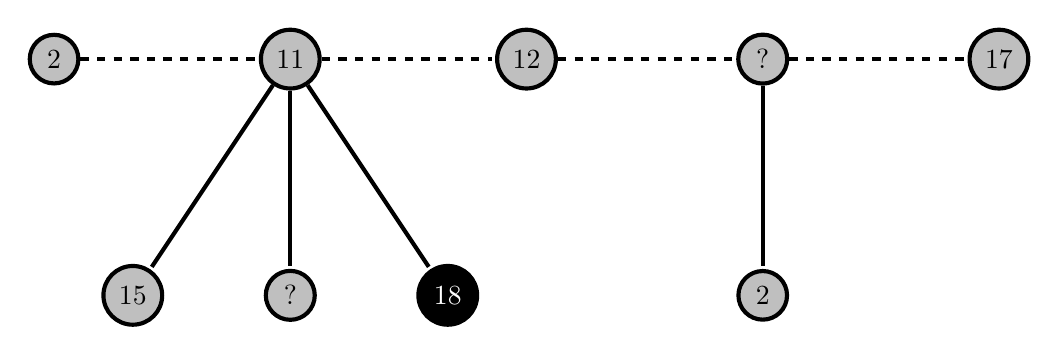
\begin{tikzpicture}[-,>=stealth,shorten >=1pt,auto,
      main node/.style={circle,draw}, line width=1.5pt]
  \node[main node,fill=lightgray] (a) at (0,0) {2};
  \node[main node,fill=lightgray] (b) at (3,0) {11};
  \node[main node,fill=lightgray] (f) at (1,-3) {15};
  \node[main node,fill=lightgray] (g) at (3,-3) {?};
  \node[main node,fill=black,text=white] (h) at (5,-3) {18};
  \node[main node,fill=lightgray] (c) at (6,0) {12};
  \node[main node,fill=lightgray] (d) at (9,0) {?};
  \node[main node,fill=lightgray] (i) at (9,-3) {2};
  \node[main node,fill=lightgray] (e) at (12,0) {17};
  \path[every node/.style={font=\small}]
  (a) edge[dashed] (b)
  (b) edge[dashed] (c)
  (c) edge[dashed] (d)
  (d) edge[dashed] (e)
  (b) edge (f)
  (b) edge (g)
  (b) edge (h)
  (d) edge (i)
  ;
  \end{tikzpicture}
  \end{center}

\optionsstart
\answer 2 \correct
\answer 6
\answer 10
\answer 14 \correct
\answer 18 \correct
\answer 22 \correct
\optionsend

\explanation{
The nodes must satisfy the min-heap property, i.e.,~the unknown node on the left must contain a value greater than or equal to its parent 11, and the unknown node on the right must contain a value less than or equal to the values of its children, i.e.,~2. Therefore, 6 and 10 are the only values that fit in neither of the nodes.
}



\question{Running time of Fibonacci heaps}
Suppose that a {\sc Fib-Heap-Extract-Min} operation is performed on a Fibonacci heap $H$ with $n$ keys as described in CLRS online Chapter 19.
Before the operation the potential function has the value $\Phi(H)$, and after the operation it has the value $\Phi(H')$, where $H'$ is the new Fibonacci heap.
What can we say with certainty about the time used by the {\sc Fib-Heap-Extract-Min} operation that transforms $H$ into $H'$?
\multipleanswers

\optionsstart
\answer The time is $O(n)$ \correct
\answer The time is $O(\lg n)$
\answer The time is $O(\lg n + \Phi(H) - \Phi(H'))$ \correct
\answer The time is $O(1 + \Phi(H) - \Phi(H'))$
\answer The time is $O(1)$
\optionsend

\explanation{The amortized analysis in CLRS shows that the time used is at most (a constant times) $\lg n + \Phi(H) - \Phi(H')$. Since $0\leq \Phi(H) \leq n$, this implies a time bound of $O(n)$, i.e.,~options 1 and 3 are correct. Options 2 and 5 are not correct if the root list is longer than $O(\lg n)$, which can happen after a sequence of insertions, since {\sc Consolidate} runs through the root list. Option 4 is not correct if there is a node of degree $\lg n$ in the root list, since {\sc Consolidate} uses time proportional to the degree but does not necessarily decrease the potential. }






\question{Rod cutting}
Consider the algorithm \textsc{Extended-Bottom-Up-Cut-Rod}, CLRS Section 14.1, page 372.
Let $n=6$ and $p=\langle
4, 4, 13, 40, 43, 49\rangle$.
Which arrays $r$ and $s$ does the algorithm return when called on input $(p,n)$?
\oneanswer
\optionsstart
\answer $r=\langle 0, 4, 8, 13, 40, 44, 48\rangle$ and $s=\langle 1, 1, 3, 4, 1, 4\rangle$
\answer $r=\langle 0, 4, 8, 13, 40, 44, 48\rangle$ and $s=\langle 1, 1, 3, 4, 1, 6\rangle$
\answer $r=\langle 0, 4, 8, 13, 40, 44, 49\rangle$ and $s=\langle 1, 1, 3, 4, 1, 4\rangle$
\answer $r=\langle 0, 4, 8, 13, 40, 44, 49\rangle$ and $s=\langle 1, 1, 3, 4, 1, 6\rangle$ \correct
%\answer $r=\langle 0, 4, 4, 13, 40, 43, 49\rangle$ and $s=\langle 1, 2, 3, 4, 5, 6\rangle$.
\optionsend
\explanation{Seen by running the algorithm by hand.}



\question{Paradigms}
Consider the following pseudocode, which takes an array $A$ and two indices $p$, $r$ as parameters.
%
\begin{codebox}
  \Procname{$\proc{MyAlgorithm}(A, p, r)$}
  \li \If $p<r$ \Do
  \li $q = \lfloor (p+ r)/2\rfloor$
  \li $x = \proc{MyAlgorithm}(A, p, q)$
  \li $y = \proc{MyAlgorithm}(A, q+1, r)$
  \li $z = \proc{MyAlgorithm}(A, p+1, r)$
  \li \Return $x+y+z$ \End
  \li \Else\Do
  \li \Return $A[p]$ \End
\end{codebox}
%
Which of the paradigms below best describes $\proc{MyAlgorithm}$?
\oneanswer
\optionsstart
\answer Divide and conquer \correct
\answer Dynamic programming
\answer Greedy algorithms
\optionsend
\explanation{The algorithm works by calling itself recursively on three smaller problem instances and then combining the results. It therefore uses divide and conquer. No results are stored, so the code does not use dynamic programming. Nor is any greedy choice made (no conditions depend on the contents of $A$), so it does not fit well with a greedy algorithm either. }



%\newpage

\question{Huffman codes}
Consider the letters a, b, c, d, e, f with the corresponding frequencies a:13, b:5, c:7, d:9, e:6, f:8.
We run Huffman's algorithm on the frequencies, as described in CLRS Section 15.3.
Which tree do we get as the result?
\oneanswer
\optionsstart
\answer \qquad \includegraphics[page=6,valign=c]{ad-problems-2024-april-figs.pdf}
\itxanswer{Tree 1}
\answer \qquad \includegraphics[page=4,valign=c]{ad-problems-2024-april-figs.pdf}
\itxanswer{Tree 2}
\answer \qquad \includegraphics[page=5,valign=c]{ad-problems-2024-april-figs.pdf}
\itxanswer{Tree 3}
\answer \qquad \includegraphics[page=3,valign=c]{ad-problems-2024-april-figs.pdf} \correct
\itxanswer{Tree 4}
\answer \qquad \includegraphics[page=7,valign=c]{ad-problems-2024-april-figs.pdf}
\itxanswer{Tree 5}
\optionsend
\explanation{Seen by running the algorithm by hand.}





\question{Red-black search trees}\label{q:red-black}
Consider a red-black binary search tree $T$, as described in CLRS Chapter 13.
Consider the tree below, where all leaves are omitted (as in CLRS Figure 13.1.c) and three internal nodes are unspecified:

\begin{center}
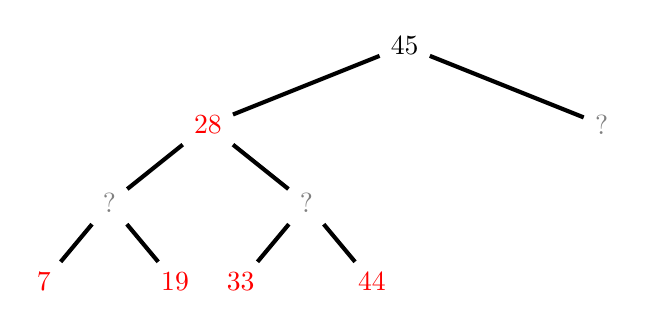
\begin{tikzpicture}[-,>=stealth,level/.style={sibling distance = 5cm/#1,
    level distance = 1cm}, line width=1.5pt]
  \node [black] {45}
      child{ node [red] {28}
              child{ node [gray] {?}
                  child{ node [red] {7} }
                  child{ node [red] {19}}
              }
              child{ node [gray] {?}
                              child{ node [red] {33}}
                              child{ node [red] {44}}
              }
      }
      child{ node [gray] {?}
          }
  ;
  \end{tikzpicture}
\end{center}

\medskip

Which nodes are possible in at least one of the positions marked with ?, if the tree must satisfy the invariants of a red-black binary search tree?
\multipleanswers
\optionsstart
\answer A red node with key 13
\answer A black node with key 17 \correct
\answer A red node with key 29
\answer A black node with key 37 \correct
\answer A red node with key 48
\answer A black node with key 84 \correct
\optionsend
\explanation{ All the marked nodes must be black. The two on the left because their parent is red. The last one because there must be the same number of black nodes on all paths from the root to the leaves. The keys 17, 37, and 84 are all consistent with the invariant that the tree is a search tree (17 lies between 7 and 19, 37 between 33 and 44, and 84 is greater than 45).
}



\question{Rotations in red-black search trees}
Consider this red-black binary search tree $T$, where the leaves are omitted from the drawing:
%
\begin{center}
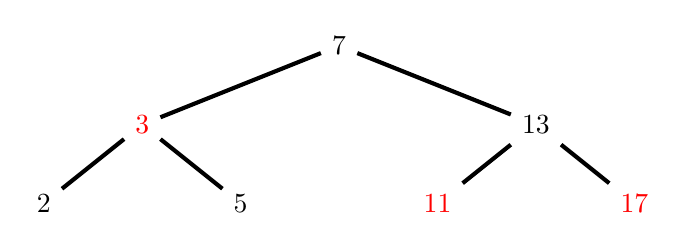
\begin{tikzpicture}[-,>=stealth,level/.style={sibling distance = 5cm/#1,
    level distance = 1cm}, line width=1.5pt]
  \node [black] {7}
      child{ node [red] {3}
              child{ node [black] {2}
              }
              child{ node [black] {5}
              }
      }
      child{ node [black] {13}
              child{ node [red] {11}
              }
              child{ node [red] {17}
              }
          }
  ;
  \end{tikzpicture}
\end{center}

\medskip

Suppose we run the algorithm {\sc Left-Rotate$(T,7)$} described in CLRS Section 13.2, that is, with the node $7$ as input.
What happens to the tree $T$?
\multipleanswers
\optionsstart
\answer 3 becomes the new root and is colored black
\answer 13 becomes the new root \correct
\answer The height stays the same
\answer The height increases by 1 \correct
\optionsend
\explanation{ {\sc Left-Rotate$(T,7)$} makes 13 the root with 7 and 17 below it. Node 11 becomes the right child of 7. No nodes change color. After the rotation, nodes 2 and 5 are one step further from the root than before.
}


\question{Minimum spanning tree}
Consider the minimum spanning tree problem on this graph:
\begin{center}
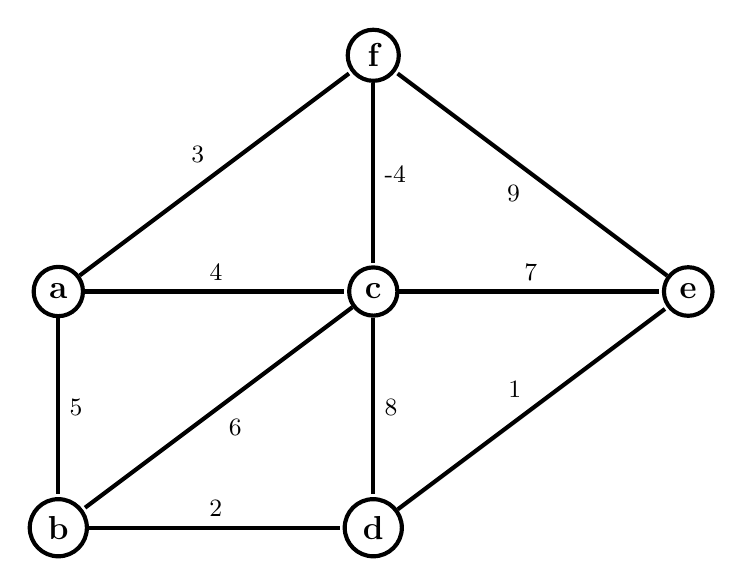
\begin{tikzpicture}[-,>=stealth,shorten >=1pt,auto,
  main node/.style={circle,draw,font=\large\bfseries}, line width=1.5pt]
\node[main node] (a) at (2,1.5) {a};
\node[main node] (b) at (2,-1.5) {b};
\node[main node] (c) at (6,1.5) {c};
\node[main node] (d) at (6,-1.5) {d};
\node[main node] (e) at (10,1.5) {e};
\node[main node] (f) at (6,4.5) {f};

\path[every node/.style={font=\small}]
(a) edge node {5} (b)
edge node {4} (c)
(b) edge node {2} (d)
(a) edge node {3} (f)
(c) edge node {8} (d)
edge node {7} (e)
edge node {6} (b)
(d) edge node {1} (e)
(e) edge node {9} (f)
(f) edge node {-4} (c);
\end{tikzpicture}
\end{center}
Which edges are in the minimum spanning tree (which is unique)?
\multipleanswers
\optionsstart
\answer \{a,b\} \correct
\answer \{a,c\}
\answer \{a,f\} \correct
\answer \{b,c\}
\answer \{b,d\} \correct
\answer \{c,d\}
\answer \{c,e\}
\answer \{c,f\} \correct
\answer \{d,e\} \correct
\answer \{e,f\}
\optionsend
\explanation{The minimum spanning tree can be found by running, e.g., Kruskal's or Prim's algorithm. Kruskal's algorithm adds the edges in order of weight, i.e.,~it starts with \{c,f\}, \{d,e\}, \{b,d\}, \{a,f\}, skips \{a,c\} because it would create a cycle, and finishes with \{a,b\}. }



\question{Cuts and safe edges}
Consider the following undirected, weighted, connected graph $G=(V,E)$ with vertex set $V = \{A,B,C,D,E,F\}$:
We are interested in light edges for an edge set $K$ in various cuts.
Which of the following statements are true for the edge set $K = \{\{D,F\},\{C,E\},\{A,B\}\}$? \multipleanswers

\begin{center}
  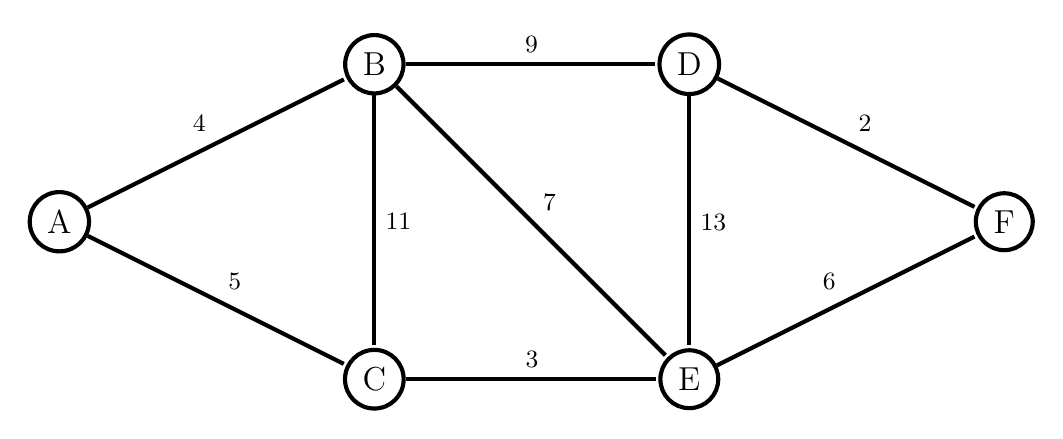
\begin{tikzpicture}[-,>=stealth,shorten >=1pt,auto,
      main node/.style={circle,draw,font=\large}, line width=1.5pt]
  \node[main node] (a) at (0,0) {A};
  \node[main node] (b) at (4,2) {B};
  \node[main node] (c) at (4,-2) {C};
  \node[main node] (d) at (8,2) {D};
  \node[main node] (e) at (8,-2) {E};
  \node[main node] (f) at (12,0) {F};
  \path[every node/.style={font=\small}]
  (a) edge node {4} (b)
  (a) edge node {5} (c)
  (b) edge node {11} (c)
  (b) edge node {9} (d)
  (b) edge node {7} (e)
  (c) edge node {3} (e)
  (d) edge node {13} (e)
  (d) edge node {2} (f)
  (e) edge node {6} (f);
  \end{tikzpicture}
  \end{center}


\optionsstart
\answer The cut $(S_1, V - S_1)$ respects the edge set $K$ for $S_1=\{A,B\}$ \correct
\answer The cut $(S_2, V - S_2)$ respects the edge set $K$ for $S_2=\{C,D,E,F\}$ \correct
\answer The cut $(S_3, V - S_3)$ respects the edge set $K$ for $S_3=\{A,B,F\}$
\answer The cut $(S_4, V - S_4)$ has $\{E,F\}$ as a light edge for $S_4=\{A,B,C,E\}$ \correct
\answer The cut $(S_5, V - S_5)$ has $\{B,D\}$ as a light edge for $S_5=\{C,D,E,F\}$
\answer The cut $(S_6, V - S_6)$ has $\{A,C\}$ as a light edge for $S_6=\{A,B,D,F\}$ \correct
\optionsend
\explanation{None of the edges incident to only one of the vertices $A$ and $B$ belongs to $K$. Therefore, the cut $(S_1,V - S_1)$ respects $K$. None of the edges incident to one of the vertices $C, D, E, F$ belongs to $K$. Therefore, the cut $(S_2,V - S_2)$ respects $K$. The edge $\{D,F\}$ has $F$ in $S_3$ and $D$ in $V - S_3$. Therefore, the cut $(S_3,V - S_3)$ does not respect $K$. The edge $\{E,F\}$ has minimum weight in the cut $(S_4, V - S_4)$ and is therefore a light edge. The edge $\{B,E\}$, which crosses $(S_5, V - S_5)$, has smaller weight than the edge $\{B,D\}$, which also crosses the same cut. $\{B,D\}$ is therefore not a light edge. The edge $\{A,C\}$ crosses the cut $(S_6, V - S_6)$ and has minimum weight in the cut; it is therefore a light edge for the cut.
}





\question{Kruskal's algorithm}
Consider the following weighted, undirected graph, where the edges of the minimum spanning tree (which is unique) are marked with bold lines:
\begin{center}
  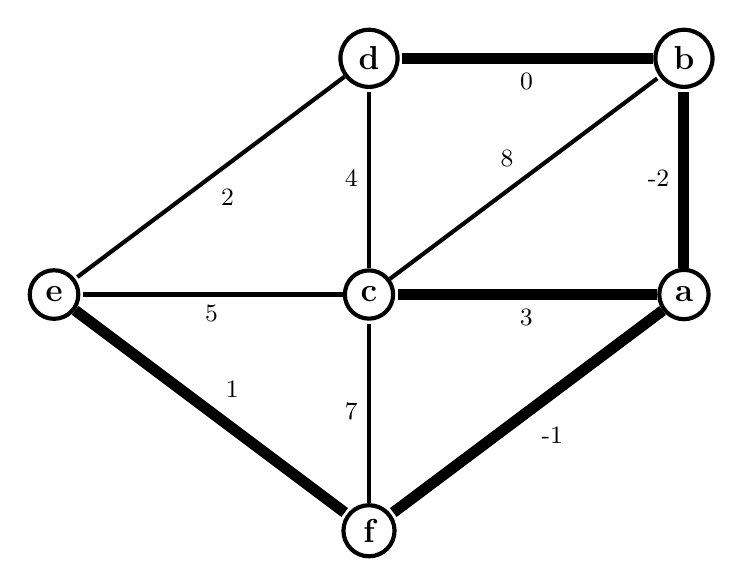
\begin{tikzpicture}[-,>=stealth,shorten >=1pt,auto,
    main node/.style={circle,draw,font=\large\bfseries}, line width=1.5pt]
  \node[main node] (a) at (-2,-1.5) {a};
  \node[main node] (b) at (-2,1.5) {b};
  \node[main node] (c) at (-6,-1.5) {c};
  \node[main node] (d) at (-6,1.5) {d};
  \node[main node] (e) at (-10,-1.5) {e};
  \node[main node] (f) at (-6,-4.5) {f};

  \path[every node/.style={font=\small}]
  (a) edge[line width=4pt] node {-2} (b)
  edge[line width=4pt] node {3} (c)
  (b) edge[line width=4pt] node {0} (d)
  (a) edge[line width=4pt] node {-1} (f)
  (c) edge node {4} (d)
  edge node {5} (e)
  edge node {8} (b)
  (d) edge node {2} (e)
  (e) edge[line width=4pt] node {1} (f)
  (f) edge node {7} (c);
  \end{tikzpicture}
\end{center}
In which order are the edges included in the minimum spanning tree when Kruskal's algorithm is run on this graph? \oneanswer
\optionsstart
\answer \{a,b\}, \{a,c\}, \{a,f\}, \{b,d\}, \{e,f\}  % Lexicographically
\answer \{a,b\}, \{a,f\}, \{b,d\}, \{e,f\}, \{a,c\} \correct
\answer \{b,d\}, \{a,f\}, \{e,f\}, \{a,b\}, \{a,c\} % By absolute value
\answer \{b,d\}, \{a,c\}, \{e,f\}, \{a,b\}, \{a,f\} % Distractor
\answer \{b,d\}, \{a,f\}, \{e,f\}, \{a,b\}, \{a,c\}  % Distractor
\optionsend
\explanation{Running Kruskal's algorithm by hand gives the stated order.}




\question{Shortest paths}
Consider the following directed, weighted graph $G=(V,E)$:
\begin{center}
  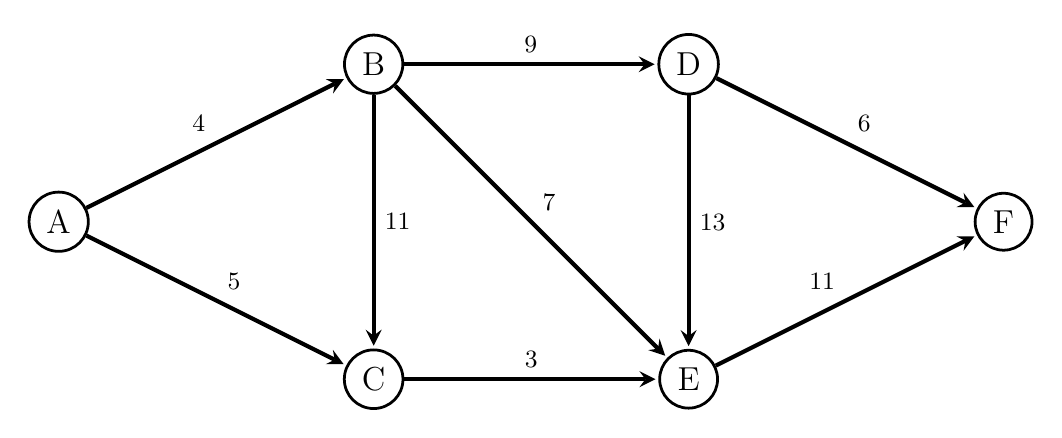
\begin{tikzpicture}[->,>=stealth,shorten >=1pt,auto,
      main node/.style={circle,draw,font=\large,line width=1pt}, line width=1.5pt]
  \node[main node] (a) at (0,0) {A};
  \node[main node] (b) at (4,2) {B};
  \node[main node] (c) at (4,-2) {C};
  \node[main node] (d) at (8,2) {D};
  \node[main node] (e) at (8,-2) {E};
  \node[main node] (f) at (12,0) {F};
  \path[every node/.style={font=\small}]
  (a) edge node {4} (b)
  (a) edge node {5} (c)
  (b) edge node {11} (c)
  (b) edge node {9} (d)
  (b) edge node {7} (e)
  (c) edge node {3} (e)
  (d) edge node {13} (e)
  (d) edge node {6} (f)
  (e) edge node {11} (f);
  \end{tikzpicture}
  \end{center}
Which edges are on a shortest path from vertex A to \emph{at least} one of the vertices \{B,C,D,E,F\}?
\multipleanswers
\optionsstart
\answer \{A,B\} \correct
\answer \{A,C\} \correct
\answer \{B,C\}
\answer \{B,D\} \correct
\answer \{B,E\}
\answer \{C,E\} \correct
\answer \{D,E\}
\answer \{D,F\} \correct
\answer \{E,F\} \correct
\optionsend
\explanation{Most edges on a shortest path are in the shortest-paths tree, which can be found, e.g., by running Dijkstra's algorithm by hand. In the last step, however, there are two possible edges into F that both result in a shortest path, so both must be included.}





\question{Choice of algorithms and data structures}
Suppose you have to solve the $k$-{\sc Difference} problem, defined as follows: Given a parameter~$k$ and an array $A$ of $n$ integers, decide whether there are two numbers in $A$ whose difference is $k$.

\medskip

\noindent
{\bf Example.} If $k=4$ and $A = \langle 2, 7, 13, 3, 11, 17\rangle$, the answer is ``yes'', because we have $A[2]-A[4] = 7 - 3 = 4$. If $k=3$ and $A$ is unchanged, the answer is ``no'', since there are no two numbers in $A$ whose difference is 3.

\medskip

\noindent
Which of the following algorithms and data structures is most relevant as part of a simple and efficient algorithm that solves $k$-{\sc Difference}?
\oneanswer

\optionsstart
\answer Dijkstra's algorithm
\answer Disjoint sets
\answer Dynamic tables
\answer Merge-sort \correct
\answer Prim's algorithm
\optionsend
\explanation{By first sorting $A$, the problem can be solved in an additional $O(n)$ time by performing a {\sc Merge} of $\langle A[1],\dots,A[n]\rangle$ and $\langle A[1]+k,\dots,A[n]+k\rangle$ and noting whether there are identical elements in the two lists. (Alternatively, one can perform $n$ binary searches for an element with value $A[i]-k$, for $i=1,\dots,n$.) In both cases the algorithm takes total time $O(n \lg n)$. The other algorithms and data structures mentioned cannot directly be used as part of a simple and efficient algorithm.}




\multiplechoiceend

\newpage


\section*{Written problems}\label{sec:written}

% Machine translated from the Danish original, ../danish/skriftlige.tex
{\bf Written problems:} \placeholder{How the answers are submitted, e.g.\ the file format and exam system, and whether drawings made on a tablet may be inserted.}
\begin{itemize}
    \item Use \emph{one page for each subquestion, in the same order as in the problem set.}
    \item The number/letter of the subquestion (e.g.\ 19 or 20.a) must be stated.
\end{itemize}





\section{Proofs by induction (7\%)}

Consider the following function, in the pseudocode notation of CLRS, where the input $A$ is an array of integers, $n$ is the length of $A$, and $b$ is an integer parameter.
\begin{codebox}
  \Procname{$\proc{HeavyHitter}(A, n, b)$}
  \li let $r[1:b]$ be a new array
  \li \For $i = 1$ \To $b$
  \li \Do $r[i] = 0$ \End
  \li \For $j = 1$ \To $n$ \Do
  \li \If $A[j]\geq 1$ and $A[j]\leq b$ \Do
  \li $r[A[j]] = r[A[j]] + 1$ \End \End
  \li \Return $\max_{1\leq\ell\leq b}(r[\ell])$
\end{codebox}

\noindent
{\bf Example:} For $n=6$, $b=10$, $A = \langle 5,1,1,7,1,3\rangle$, {\sc HeavyHitter} returns the value $3$.
\medskip

\subquestion{a)}{ Explain in words what {\sc HeavyHitter} computes.}

\explanation{ {\sc HeavyHitter} computes how many times the most frequent element of $A$ occurs, where elements of $A$ that do not lie in the interval $[1,\dots,b]$ are ignored. }


\subquestion{b)}{ Formulate a loop invariant $I(j)$ that describes the contents of $r$ after iteration~$j$ of the {\bf for} loop in lines 4--6.
Argue by induction that the invariant holds after $j$ iterations, for $j\geq 0$.
The invariant $I(n)$, which holds when the loop terminates, should support your answer to question {\bf a)}.}

\explanation{ Invariant $I(j)$: For $i\in\{1,\dots,b\}$ we have $r[i] = |\{ k \; | \; 1\leq k \leq j \wedge A[k]=i \}|$.
The invariant holds for $j=0$ since $r[i]=0$ (because of the initialization in lines 2-3).
In the inductive step we assume $I(j-1)$ and want to show that $I(j)$ holds after iteration $j$.
The value of $r[i]$ is increased by 1 in iteration $j$ exactly if $A[j]=i$, and the same holds for $|\{ k \; | \; 1\leq k \leq j \wedge A[k]=i \}|$.
}


\section{As long as possible (12\%)}

We consider the following variant of the activity-selection problem from CLRS Section 15.1.
Instead of maximizing the number of activities as in CLRS, we want to select a set of activities whose total duration is \emph{as long as possible}.
That is, we are given a set $S=\{a_1,a_2,\ldots,a_n\}$ of $n$ elements, where each activity $a_i$ has a given start time $s_i$ and a finish time $f_i$, with $0\leq s_i<f_i<\infty$.
Assume that the activities are sorted by finish time, i.e.,~$f_1\leq f_2\leq\cdots\leq f_n$.
We want to select a set $A\subseteq S$ of non-overlapping activities that maximizes $\sum_{a_i\in A} (f_i-s_i)$.
That the activities in $A$ are non-overlapping means that if $a_i,a_j\in A$ with $i\neq j$, then $[s_i,f_i)\cap [s_j,f_j)=\emptyset$, i.e.,~it is allowed that $f_i = s_j$ or $f_j = s_i$.

\subquestion{a)}{
Suppose the activities are $S=\{a_1,a_2,a_3,a_4\}$ with start times $s=\langle 0,3,1,6\rangle$ and finish times $f=\langle 2,4,5,8\rangle$.
Give an optimal solution $A$.}

\explanation{The optimal solution is $\{a_3,a_4\}$, which has total duration $6$.
\medskip}

For each $i\in\{0, 1,\ldots,n\}$, let $S_i=\{a_1,a_2,\ldots,a_i\}$ be the set consisting of the first $i$ activities, i.e.,~$S_0=\emptyset$, $S_1=\{a_1\}$, $S_2=\{a_1, a_2\}$, etc.
Define $t_i$ to be the total time of the activities in an optimal solution for $S_i$, where in particular $t_0=0$.

\subquestion{b)}{
  Consider a fixed index $i\in\{1,\ldots,n\}$ and let $j\in\{0,1,\ldots,i-1\}$ be the largest index such that $f_j\leq s_i$ (here we define $f_0=0$).
  Argue that
\[
t_i=\max\{t_{i-1},t_j+f_i-s_i\}.
\]}

\explanation{Either the optimal solution for $S_i$ includes the activity $a_i$, or it does not.
In the first case, in addition to $a_i$ we must choose an optimal solution among the activities that finish no later than when $a_i$ starts, that is, among $S_j$, where $j$ is defined as in the problem statement.
In the second case, the solution must be the same as the optimal one for $S_{i-1}$, that is, $t_{i-1}$.
This shows that $t_i\leq \max\{t_{i-1},t_j+f_i-s_i\}$.
Both candidates are valid solutions for $S_i$, so we also have $t_i\geq \max\{t_{i-1},t_j+f_i-s_i\}$.
Therefore, $t_i=\max\{t_{i-1},t_j+f_i-s_i\}$.
}

\subquestion{c)}{
Write pseudocode for an algorithm that returns the total time $t_n$ of the activities in the optimal solution for the entire set $S$.
The signature of your pseudocode must be
\[\textsc{Activity-Selection-Max-Span}(s,f,n),\]
where $s$ and $f$ are arrays of length $n$ containing the start and finish times, respectively.
To get full points the algorithm must have running time $O(n^2)$, but it is not necessary to prove the bound on the running time.}

\explanation{By part b) we can use dynamic programming.
Here is a possible solution:

\medskip

\textsc{Activity-Selection-Max-Span}$(s,f,n)$

\quad Let $t[0:n]$ be a new array.

\quad $t[0]=0$

\quad for $i=1$ to $n$

\quad\quad Use binary search to find the max.~$j\in\{0,1,\ldots,i-1\}$ such that $j==0$ or $f[j]\leq s[i]$.

\quad\quad $t[i]=\max\{t[i-1],t[j]+f[i]-s[i]\}$

\quad return $t[n]$
}

\subquestion{d)}{
Explain how to design an algorithm that solves the problem in $O(n \lg n)$ time.
If your algorithm from problem c) already has this running time, argue why.}

\explanation{The algorithm from question c) has running time $O(n \lg n)$ because the for loop iterates over $n$ values and we spend $O(\lg n)$ time on binary search in each iteration.}



\section{As many as possible (9\%)}\label{sec:last}

We consider an array of $n$ integers $X=\langle x_1,x_2,\ldots,x_n\rangle$, where $x_i$ can be positive, negative, or $0$.
Let $S=\sum_{i=1}^n x_i$ be the sum of the numbers.
We want to solve the {\sc Longest-Subset-Sum} problem:
Find the size of the largest index set $I\subseteq \{1,2,\ldots, n\}$ such that $\sum_{i\in I} x_i\leq S/2$.

\medskip
{\bf Example.} For $X=\langle 1,4,2,8\rangle$, which has $S=15$, we can find a set $I$ with~3 elements, namely $I=\{1,2,3\}$. This is the largest possible set satisfying $\sum_{i\in I} x_i\leq S/2$, since no solution can contain all four elements.


\subquestion{a)}{Give an example of an array $X$ for which the solution is not unique, i.e.,~where there are two \emph{different} index sets $I_1$ and $I_2$ of the largest possible size such that $\sum_{i\in I_1} x_i\leq S/2$ and $\sum_{i\in I_2} x_i\leq S/2$.}

\explanation{Example: $X=\langle 1,1\rangle$ has two optimal solutions: $I=\{1\}$ and $I=\{2\}$, both of size 1. }

\medskip

We now consider the following approach to solving {\sc Longest-Subset-Sum}: Start with the sum of all numbers in~$X$ and remove one number at a time in reverse sorted order as long as the sum is greater than~$S/2$. Return the number of elements that have not been removed from $X$.

\medskip
{\bf Example.} For $X=\langle 4, -2, -3, 2, 5, 5\rangle$, which has sum $S=11$, we remove the two largest elements $5$ and $5$, after which the sum of the four remaining numbers is 1, which is less than or equal to $S/2$. Therefore, 4 is returned.

\subquestion{b)}{
Prove that an optimal solution to {\sc Longest-Subset-Sum} can be constructed as described above.}

\explanation{
Assume that $X$ is sorted in non-decreasing order, so the proposed algorithm removes the numbers from the sum in the order $x_n,x_{n-1},\ldots,x_1$.
Consider an arbitrary index set $I^*\subseteq \{1,2,\ldots, n\}$ that gives an optimal solution, let $k=\mid I^*\mid$ be the number of numbers in $I^*$, and let $I=\{1,2,\ldots,k\}$.
If $I^*\neq I$, then $I$ gives a sum that is at most as large as that of $I^*$, so $I$ is also an optimal index set.
Since $I$ is optimal, we have $\sum_{i=1}^{k'} x_i>S/2$ for every $k'\in\{k+1,\ldots,n\}$.
Therefore, the proposed algorithm finds the optimal number $k$.}

\subquestion{c)}{Write pseudocode for an algorithm that solves {\sc Longest-Subset-Sum}.
The signature of your algorithm must be \[\textsc{Longest-Subset-Sum}(x,n),\]
where $x$ is an array of length $n$.}

\explanation{By part b), a simple greedy algorithm gives an optimal solution. The pseudocode could, for example, look as follows:

\textsc{Longest-Subset-Sum}$(x,n)$

\quad Sort $x$ in non-decreasing order, for instance using \textsc{Merge-Sort}.

\quad Let $S$ be the sum of the numbers in $x$.

\quad $R=S$

\quad $i=n$

\quad while $R>S/2$

\quad\quad $R = R - x[i]$

\quad\quad $i=i-1$

\quad return $i$
}



\label{page:last}
